\par A continuaci\'on vamos a analizar resultados para el algoritmo GeM en el contexto de la Primera Divis\'on de la Liga Argentina de F\'utbol enfoc\'andonos en el ranking de equipos y experimentando sobre variaciones del ranking est\'andar, obtenci\'on del ranking mediante el m\'etodo GeM y m\'etodos alternatvos. Tomaremos como informaci\'on de entrada el campeonato 2015 hasta la fecha 26 inclusive. 
\bigskip

\par Contamos con el ranking oficial (est\'andar) de la liga que consta de ordenar los equipos por puntaje obtenido. Por cada partido ganado un equipo suma 3 puntos, por cada partido empatado obtiene tan solo 1, mientras que no obtiene puntos si fue derrotado. Como se puede ver el ranking no toma como informaci\'on relevante los goles. Mas adelante veremos que el m\'etodo GeM se basa fuertemente en los goles pero no diferencia entre victorias y derrotas tan notoriamente como si lo hace el ranking est\'andar.

\subsection{Experimento 1}
\par Como primer experimento vamos a comparar el ranking obtenido tras la aplicaci\'on del m\'etodo GeM y el ranking est\'andar tomando como entrada los resultados de todos los partidos hasta la fecha 26 inclusive. Creemos que van a notarse diferencias sobre todo por dos motivos:
\begin{itemize}
	\item El m\'etodo GeM no tiene en cuenta los empates, resultado que se da con frecuencia en el futbol argentino;
	\item El m\'etodo GeM solo se enfoca en los goles, mientras que el m\'etodo est\'andar solo se enfoca en quien gan\'o/empat\'o/perdi\'o.
\end{itemize}

\newpage

\subsubsection{Resultados del Experimento 1}

\begin{multicols}{2}
\center
\begin{tabulary}{0.45\textwidth}{| c | c | c | c | c |}
\hline
& \textbf{Equipo} & \textbf{Puntos} \\ \hline
1 & Boca Juniors & 58\\ \hline
2 & San Lorenzo & 54\\ \hline
3 & Rosario Central & 52\\ \hline
4 & Racing Club & 49\\ \hline
5 & River Plate & 48\\ \hline
6 & Independiente & 45\\ \hline
7 & Banfield & 43\\ \hline
8 & Belgrano & 43\\ \hline
9 & Estudiantes (LP) & 42\\ \hline
10 & Tigre & 42\\ \hline
11 & Quilmes & 39\\ \hline
12 & Lanús & 38\\ \hline
13 & Unión & 38\\ \hline
14 & Gimnasia y Esgrima (LP) & 37\\ \hline
15 & Newell's Old Boys & 33\\ \hline
16 & San Martín (SJ) & 32\\ \hline
17 & Aldosivi & 30\\ \hline
18 & Sarmiento & 30\\ \hline
19 & Argentinos Juniors & 29\\ \hline
20 & Olimpo & 29\\ \hline
21 & Temperley & 29\\ \hline
22 & Defensa y Justicia & 27\\ \hline
23 & Huracán & 26\\ \hline
24 & Vélez Sarsfield & 26\\ \hline
25 & Godoy Cruz & 25\\ \hline
26 & Colón & 24\\ \hline
27 & Arsenal & 23\\ \hline
28 & Atlético de Rafaela & 22\\ \hline
29 & Nueva Chicago & 17\\ \hline
30 & Crucero del Norte & 14\\ \hline
\end{tabulary}
\bigskip

Ranking mediante m\'etodo est\'andar.

\columnbreak

\begin{tabulary}{0.45\textwidth}{ | c | c | c |}
\hline
& \textbf{Equipo} & \textbf{Numero}\\ \hline
1 & Boca Juniors & 0.0860189\\ \hline
2 & Aldosivi & 0.0653536\\ \hline
3 & River Plate & 0.0634998\\ \hline
4 & San Lorenzo & 0.0620352\\ \hline
5 & Rosario Central & 0.0484731\\ \hline
6 & Racing Club & 0.0478783\\ \hline
7 & San Martín (SJ) & 0.0439558\\ \hline
8 & Quilmes & 0.0423821\\ \hline
9 & Newell's Old Boys & 0.0382332\\ \hline
10 & Vélez Sarsfield & 0.0376689\\ \hline
11 & Independiente & 0.0365646\\ \hline
12 & Belgrano & 0.0363978\\ \hline
13 & Gimnasia y Esgrima (LP) & 0.0335849\\ \hline
14 & Banfield & 0.0307372\\ \hline
15 & Estudiantes (LP) & 0.0295322\\ \hline
16 & Unión & 0.0288744\\ \hline
17 & Tigre & 0.0273356\\ \hline
18 & Sarmiento & 0.026108\\ \hline
19 & Huracán & 0.0246666\\ \hline
20 & Defensa y Justicia & 0.023737\\ \hline
21 & Lanús & 0.022729\\ \hline
22 & Olimpo & 0.0224689\\ \hline
23 & Arsenal & 0.0208702\\ \hline
24 & Godoy Cruz & 0.017516\\ \hline
25 & Temperley & 0.016045\\ \hline
26 & Crucero del Norte & 0.0160393\\ \hline
27 & Argentinos Juniors & 0.0153984\\ \hline
28 & Nueva Chicago & 0.0142318\\ \hline
29 & Atlético de Rafaela & 0.0113878\\ \hline
30 & Colón & 0.0102765\\ \hline
\end{tabulary}
\bigskip

Ranking mediante m\'etodo GeM.
\end{multicols}

\par En los resultados se puede observar que hay variaciones en las posiciones de los distintos equipos. Esto era de esperarse porque los m\'etodos usados se enfocan en distintos aspectos.
\bigskip

\par Vamos a analizar el caso particular de Aldosivi. En el ranking est\'andar se encuentra en la posici\'on 17, consecuencia de tan solo haber ganado 8 partidos y empatar 6 sobre 26 jugados. Mientras que en el ranking GeM se posiciona en el segundo lugar, veamos por qu\'e sucede esto. Recordemos que el m\'etodo GeM cuenta la diferencia de goles para con su rival en sus partidos ganados. Aldosivi, en los 8 partidos ganados no recibi\'o goles y convirti\'o 15. Cuenta entonces con una diferencia de goles importante, que lo posiciona en segundo lugar.

\par Con este claro ejemplo podemos ver la diferencia de enfoques de los dos m\'etodos. Creemos que para un deporte como el futbol el m\'etodo de GeM no est\'a bien formulado y no se enfoca en los resultados finales. Tal vez en otras ligas donde la diferencia de goles entre el ganador y el perdedor sea mayor (como la española o la alemana) y se den pocos empates pueda acercarse mas al m\'etodo est\'andar y/o competir con \'el sobre cu\'al deber\'ia ser el oficial.

\newpage

\subsection{Experimento 2}

\par Luego de analizar los resultados del experimento 1 queremos ver mas en detalle la influencia de los empates en el ranking obtenido por el m\'etodo GeM. Sabemos que al no tener en cuenta estos resultados nos alejamos del ranking est\'andar, pero queremos determinar si es factible que con alg\'un tipo de modificaci\'on podamos ajustarlo a un deporte con empates recurrentes (en este caso el f\'utbol).
\par Para tomar en consideraci\'on a los empates vamos a igualarlos a una victoria 1 a 0: ``empate = victoria por 1 a 0''. Sabemos que \'esto influye positivamente sobre los equipos con muchos empates, pero al darle un resultado favorable m\'inimo (1 a 0) creemos que no afectar\'a demasiado, manteniendo as\'i la base del enfoque del m\'etodo GeM y d\'andole cierta importancia a los empates.

\subsubsection{Resultados del Experimento 2}

\begin{figure}[ht]
\begin{center}
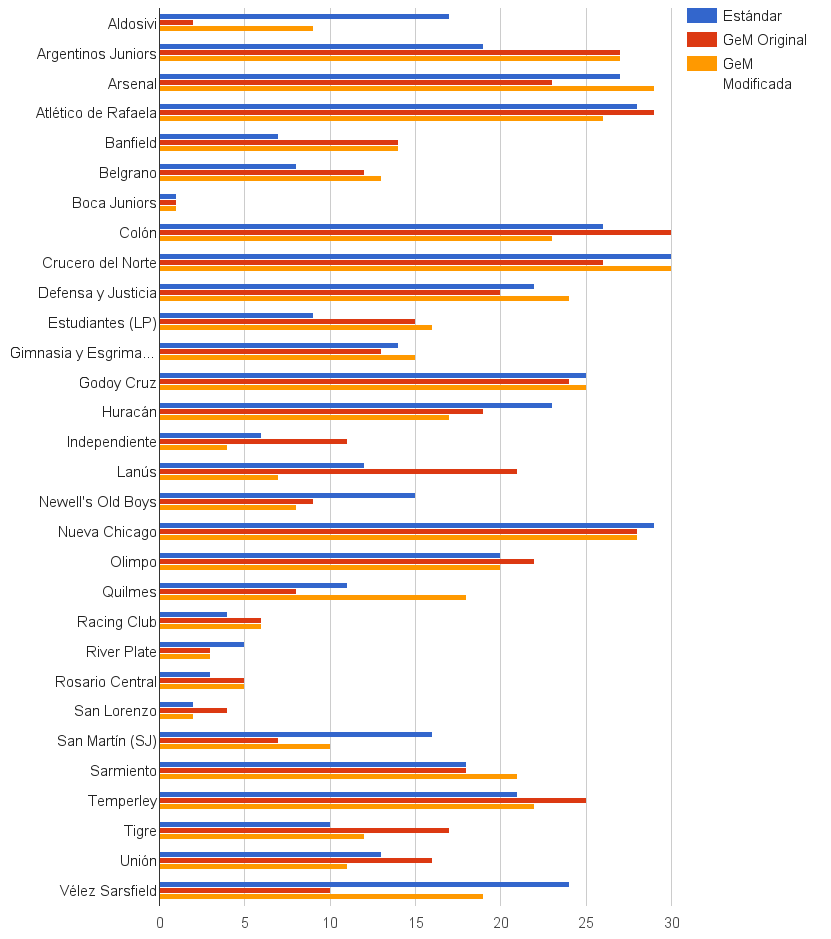
\includegraphics[width=0.7\columnwidth]{../src/experimentos/deportivos/2/experimento2.png}
\caption{Comparaciones de Rankings}
\end{center}
\end{figure}

\par En los resultados obtenidos vemos que la modificaci\'on del m\'etodo GeM gener\'o cambios en el posicionamiento de los equipos con empates en su historial. En algunos casos estos cambios lo alejaron de su posicionamiento en el ranking est\'andar mientras que en la mayor\'ia de los casos lo acercaron, d\'andole as\'i un cierto valor al empate que antes no era tenido en cuenta. Como nombramos antes, mantuvimos el enfoque del m\'etodo GeM pero le agregamos un pequeño valor a los empates que los gener\'o una tabla que creemos mas adecuada a la realidad del f\'utbol.

\newpage

\begin{multicols}{2}
\center
\begin{tabulary}{0.45\textwidth}{| c | c | c | c | c |}
\hline
& \textbf{Equipo} & \textbf{Puntos} \\ \hline
1 & Boca Juniors & 58\\ \hline
2 & San Lorenzo & 54\\ \hline
3 & Rosario Central & 52\\ \hline
4 & Racing Club & 49\\ \hline
5 & River Plate & 48\\ \hline
6 & Independiente & 45\\ \hline
7 & Banfield & 43\\ \hline
8 & Belgrano & 43\\ \hline
9 & Estudiantes (LP) & 42\\ \hline
10 & Tigre & 42\\ \hline
11 & Quilmes & 39\\ \hline
12 & Lanús & 38\\ \hline
13 & Unión & 38\\ \hline
14 & Gimnasia y Esgrima (LP) & 37\\ \hline
15 & Newell's Old Boys & 33\\ \hline
16 & San Martín (SJ) & 32\\ \hline
17 & Aldosivi & 30\\ \hline
18 & Sarmiento & 30\\ \hline
19 & Argentinos Juniors & 29\\ \hline
20 & Olimpo & 29\\ \hline
21 & Temperley & 29\\ \hline
22 & Defensa y Justicia & 27\\ \hline
23 & Huracán & 26\\ \hline
24 & Vélez Sarsfield & 26\\ \hline
25 & Godoy Cruz & 25\\ \hline
26 & Colón & 24\\ \hline
27 & Arsenal & 23\\ \hline
28 & Atlético de Rafaela & 22\\ \hline
29 & Nueva Chicago & 17\\ \hline
30 & Crucero del Norte & 14\\ \hline
\end{tabulary}
\bigskip

Ranking mediante m\'etodo est\'andar.

\columnbreak

\begin{tabulary}{0.4\textwidth}{ | c | c | c |}
\hline
& \textbf{Equipo} & \textbf{Numero}\\ \hline
1 & Boca Juniors & 0.0532173\\ \hline
2 & San Lorenzo & 0.0466695\\ \hline
3 & River Plate & 0.0466113\\ \hline
4 & Independiente & 0.0443246\\ \hline
5 & Rosario Central & 0.0436734\\ \hline
6 & Racing Club & 0.0391814\\ \hline
7 & Lanús & 0.0385408\\ \hline
8 & Newell's Old Boys & 0.0383858\\ \hline
9 & Aldosivi & 0.0381275\\ \hline
10 & San Martín (SJ) & 0.0370988\\ \hline
11 & Unión & 0.0370056\\ \hline
12 & Tigre & 0.0347199\\ \hline
13 & Belgrano & 0.0340198\\ \hline
14 & Banfield & 0.0340106\\ \hline
15 & Gimnasia y Esgrima (LP) & 0.0326107\\ \hline
16 & Estudiantes (LP) & 0.0319726\\ \hline
17 & Huracán & 0.0312592\\ \hline
18 & Quilmes & 0.0308084\\ \hline
19 & Vélez Sarsfield & 0.0306859\\ \hline
20 & Olimpo & 0.0304997\\ \hline
21 & Sarmiento & 0.0302557\\ \hline
22 & Temperley & 0.0277299\\ \hline
23 & Colón & 0.0267565\\ \hline
24 & Defensa y Justicia & 0.0262358\\ \hline
25 & Godoy Cruz & 0.024695\\ \hline
26 & Atlético de Rafaela & 0.024516\\ \hline
27 & Argentinos Juniors & 0.023696\\ \hline
28 & Nueva Chicago & 0.023149\\ \hline
29 & Arsenal & 0.0230411\\ \hline
30 & Crucero del Norte & 0.0165022\\ \hline
\end{tabulary}
\bigskip

Ranking obtenido por el m\'etodo GeM modificado.
\end{multicols}

\par Haciendo referencia al experimento 1, donde supimos comparar el ranking est\'andar del obtenido por el m\'etodo GeM, podemos sumar los resultados obtenidos con el m\'etodo GeM modificado. Notamos que las similitudes son mayores  a pesar de mantener distancia en los enfoques.

\newpage

\subsection{Experimento 3}

\par En este experimento analizaremos el impacto de la variación del parámetro $c$ sobre los resultados de rankings de competencias deportivas usando GeM. Vimos, por resultados anteriores, que aumentar el $c$ hace que el algoritmo se vuelva más lento, ya que tarda más en converger, pero devuelve resultados más justos. En este experimento nos centraremos en las diferencias entre los resultados y no en el tiempo de ejecución (ver Experimento 3 de la sección de resultados para Páginas Web).

\par Para llevar a cabo el experimento compararemos las tablas de posiciones obtenidas por cada equipo para ciertos valores de $c$, comparándolas con la posición actual en el ranking de la AFA.

\subsubsection{Resultados del Experimento 3}

\par Observemos la comparación entre las posiciones obtenidas por los equipos según cada $c$:

\begin{tabulary}{\textwidth}{| c | c | c | c | c | c | c |}
\hline						
\textbf{Pos. AFA} & \textbf{Equipo} & \textbf{c=0.85} & \textbf{c=0.65} & \textbf{c=0.45} & \textbf{c=0.25} & \textbf{c=0.00}\\ \hline
1 & Boca Juniors & 1 & 1 & 1 & 1 & 1 \\ \hline
2 & San Lorenzo & 4 & 3 & 2 & 2 & 1\\ \hline
3 & Rosario Central & 5 & 6 & 6 & 5 & 1\\ \hline
4 & Racing Club & 6 & 5 & 5 & 4 & 1\\ \hline
5 & River Plate & 3 & 2 & 3 & 3 & 1\\ \hline
6 & Independiente & 11 & 9 & 9 & 8 & 1\\ \hline
7 & Banfield & 14 & 14 & 13 & 13 & 1\\ \hline
8 & Belgrano & 12 & 11 & 10 & 9 & 1\\ \hline
9 & Estudiantes (LP) & 15 & 15 & 16 & 16 & 1\\ \hline
10 & Tigre & 17 & 15 & 15 & 14 & 1\\ \hline
11 & Quilmes & 8 & 7 & 7 & 7 & 1\\ \hline
12 & Lanús & 21 & 19 & 18 & 14 & 1\\ \hline
13 & Unión & 16 & 16 & 17 & 18 & 1\\ \hline
14 & Gimnasia y Esgrima (LP) & 13 & 13 & 12 & 12 & 1\\ \hline
15 & Newell's Old Boys & 9 & 10 & 11 & 11 & 1\\ \hline
16 & San Martín (SJ) & 7 & 8 & 8 & 10 & 1\\ \hline
17 & Aldosivi & 2 & 4 & 4 & 6 & 1\\ \hline
18 & Sarmiento & 18 & 18 & 19 & 19 & 1\\ \hline
19 & Argentinos Juniors & 27 & 26 & 25 & 25 & 1\\ \hline
20 & Olimpo & 22 & 23 & 23 & 23 & 1\\ \hline
21 & Temperley & 25 & 25 & 26 & 26 & 1\\ \hline
22 & Defensa y Justicia & 20 & 21 & 22 & 22 & 1\\ \hline
23 & Huracán & 19 & 20 & 20 & 20 & 1\\ \hline
24 & Vélez Sarsfield & 10 & 12 & 14 & 17 & 1\\ \hline
25 & Godoy Cruz & 24 & 24  & 24 & 24 & 1\\ \hline
26 & Colón & 30 & 30 & 30 & 30 & 1\\ \hline
27 & Arsenal & 23 & 22 & 21 & 21 & 1\\ \hline
28 & Atlético de Rafaela & 29 & 29 & 29 & 29 & 1\\ \hline
29 & Nueva Chicago & 28 & 28 & 28 & 28 & 1\\ \hline
30 & Crucero del Norte & 26 & 27 & 27 & 27 & 1\\ \hline
\end{tabulary}

\hspace{1cm}

\par Para las fechas del torneo de la AFA, no se ven grandes cambios en los resultados obtenidos variando el $c$ excepto en los casos de Lanús, y Vélez. Esto es una diferencia con el contexto de Páginas Web, ya que como las matrices de Markov de las competencias de fútbol no son esparsas (todos juegan contra todos), a diferencia del caso de las páginas web, no se nota tanto el impacto de la teletransportación. Sin embargo, como vimos en experimentos anteriores, debido a las diferencias de modelado del empate no podemos comparar cualitativamente si los resultados son más justos. 
\par Además, podemos ver que al disminuir el $c$ las distribuciones del vector estacionario se vuelven más equitativas, siendo el caso extremo $c = 0$, donde como se ve en la tabla, todos los equipos terminan en la misma posición.

